\chapter{Theory}

This chapter describe the theory involved in designing and imaging an \gls{odt}. The energy levels of rubidium are briefly discussed to lay a groundwork for theory and discussions on trapping and imaging. The \gls{caes}'s method of electron generation is also discussed so to provide a context for electron beam metrics and considerations. The theory of \glspl{odt} and some simulations as well as cold atom imaging methods as described here are the core of the project.

\section{Energy Levels of Rubidium}

\Gls{mot} rely on a closed transition in order to trap atoms into an atomic cloud. The \Gls{odt} and the absorption imaging scheme interact with the atoms via this same transition. The various energy levels and transitions involved are shown in figure \ref{fig:energy_levels}.

\begin{figure}[h]
\centering
%\hspace{10pt}
\begin{tikzpicture}[scale=1.5]
    \begin{scope}[thick, decoration={snake,amplitude=.4mm,
        segment length=2mm,post length=1mm}]

    % 5 2S 3/2
        \draw (-0.5, 0.05) node {$5 ^2 S_{3/2}$};
        \draw (0, -0.1) -- (4, -0.1) node[right=0.5 cm] {F=2};
        \draw (0, 0.2) -- (4, 0.2) node[right=0.5 cm] {F=3};
    % 5 2P1/2
        \draw (-0.5, 1.0) node {$5 ^2 P_{1/2}$};
        \draw (0, 1.0) -- (4, 1.0) node[right=0.5 cm] {F=4, 3, 2, 1};        
    % 5 2P3/2
        \draw (-0.5, 2.45) node {$5 ^2 P_{3/2}$};
        \draw (0, 1.9) -- (4, 1.9) node[right=0.5 cm] {F=1};
        \draw (0, 2.2) -- (4, 2.2) node[right=0.5 cm] {F=2};
        \draw (0, 2.6) -- (4, 2.6) node[right=0.5 cm] {F=3};
        \draw[dotted] (0, 2.8) -- (4, 2.8);
        \draw (0, 3.0) -- (4, 3.0) node[right=0.5 cm] {F=4};
    % Photons - cycling transition
        \draw (0.6, 3.4) node[anchor=north] {Cooling};
        \draw[decorate,red,-triangle 60] (0.5,0.2) -- (0.5, 2.8);
        \draw[decorate,red,-triangle 60] (0.7, 3.0) -- (0.7,0.2);
    % Forbidden Transitions
        \draw (2.0, 3.4) node[anchor=north] {Forbidden};
        \draw[decorate,green,-triangle 60] (1.9,3.0) -- (1.9, 1.0);
        \draw[decorate,green,-triangle 60] (2.1,3.0) -- (2.1, -0.1);
    % Dark/repump
        \draw (3.4, 3.4) node[anchor=north] {Repump};
        \draw[decorate,blue,-triangle 60] (3.3,2.6) -- (3.3, -0.1);
        \draw[decorate,blue,-triangle 60] (3.5,-0.1) -- (3.5, 2.6);
    \end{scope}
\end{tikzpicture}
\caption[Title]{The energy levels involved in trapping rubidium in a MOT. The first two transitions show the cycling transition that is used by the main cooling lasers in a MOT. The third and fourth red lines show two forbidden transitions. If the cooling laser excites to the F=3 level then it is possible for the atom to decay to the `dark' F=2 state. The repump laser serves to restore these atoms to the cycle. The dotted line indicates the detuning required for Doppler cooling.}
\label{fig:energy_levels}
\end{figure}

The $5 ^2 S_{3/2}\;F=3\rightarrow5 ^2 P_{3/2}\;F=4$ transition in rubidium forms a closed loop. Atoms are excited to the F=4 state and then spontaneously decay back to the F=3 state. The atom is forbidden to decay into any of the $5 ^2 P_{1/2}$ states since such a transition would not conserve parity. The excited atoms are also forbidden to decay via a dipole transition to the $5 ^2 S_{3/2}\;F=2$ state since this would require an angular momentum change of 2 which a single photon cannot supply

There is a small chance that an atom absorbing a photon will be excited to the F=3 state after which the atom can decay to either the F=3 ground state or the F=2 `dark' state. If the atoms enters the `dark' state then it no longer interacts with the cooling beams and thus is no longer trapped. A repump laser is tuned to the $5 ^2 S_{3/2}\;F=2\rightarrow5 ^2 P_{3/2}\;F=3$ transition so that these atoms can be reintroduced to the cycling transition and remain trapped.

\section{Electron Generation in the Cold-Atom Electron Source}
The \gls{caes} uses two-stage photoionisation as its primary method of electron production. This method provides good control over the excess energy of the ionised electrons which is essential to the production of cold electrons. Control of the initial electron bunch shape is also possible by using a \gls{slm} as described by McCulluch et al.\cite{mcculloch_arbitrarily_2011}.

Two lasers with different wavelengths can be used for efficient ionisation of atoms while producing cold electrons. An excitation laser takes the atoms from the ground state to an intermediary excited state and an ionisation laser takes the excited atoms from the intermediary state to the ionisation continuum. The excess energy of the ionised electrons can be controlled by varying the wavelength of the ionisation laser.

\begin{figure}[h]
\hspace{0.235\textwidth}
\begin{tikzpicture}[scale=1.5]
    \begin{scope}[thick, decoration={snake,amplitude=.4mm,
        segment length=2mm,post length=1mm}]
      \draw (0, 0) node[left=0.4cm] {\large $\ket{g}$}
        -- (2, 0);
      \draw (0, 1.5)  node[left=0.4cm] {\large $\ket{e}$}
        -- (2, 1.5);

      \draw (0, 2.5) -- (2, 2.5);
      \draw (0, 3) -- (2, 3);
      \draw (0, 3.25) -- (2, 3.25);
      \draw (0, 3.375) node[left=0.4cm] {Rydberg states} -- (2, 3.375);
      \draw[style=dashed] (0, 3.4375) -- (2, 3.4375);
      \draw (0, 3.5) -- (2, 3.5);
      \shade[top color=white,bottom color=black] (0, 3.5) rectangle
        node[above=0.1] {Continuum} (2, 3.75);

      \draw[decorate,red,-triangle 60] (1,0) -- ++(90:1.5);% excitation
      \draw[decorate,blue,-triangle 60] (1,1.5) -- (1, 3.4375);% ionisation

      \draw (1, 0.75) node[left=0.25cm] {$\hbar\omega_1$};
      \draw (1, 2) node[left=0.25cm] {$\hbar\omega_2$};
    \end{scope}
\end{tikzpicture}
\caption[Title]{Energy level diagram for an atom undergoing two-stage ionisation. Resonant excitation from the ground state, $\ket{g}$, to the excited state, $\ket{e}$, is achieved with a coupling laser of frequency $\omega_1$. A second laser of frequency $\omega_2$ is used to couple $\ket{e}$ to a Rydberg state or the ionisation continuum. The atom can then be field ionised from the Rydberg state by the uniform electric field.}
\label{fig:energy_level}
\end{figure}

In the \gls{caes} the excitation laser is resonant to the D2 transition of the trapped $^{85}$Rb atoms ($780.24\,\unit{nm}$). This resonance results in efficient population transfer to the excited state. The ionisation laser can be set to couple the first excited state to a Rydberg state rather than to the ionisation continuum directly which results in resonant transitions. The resonant transition to a Rydberg state followed by field ionisation induced by the accelerating electric field (see figure \ref{fig:field_ionisation}) is more efficient than other ionisation pathways which rely on non-resonant behaviour. Field ionisation results in free electrons with very little energy ($T\approx10\,\unit{K}$\cite{mcculloch_arbitrarily_2011}) and are thus `cold'.

\begin{figure}[h]
\centering
\begin{tikzpicture}[scale=2]
    \begin{scope}[thick, decoration={snake,amplitude=.4mm,
        segment length=2mm,post length=1mm}]
    \filldraw[fill=blue] (0, 1.9) circle (0.05);
    \draw [color=black, dotted] (-1.4, 1.9) -- (1.4, 1.9);
    \draw (0, 1) node {\small No electric field};
    \draw [dashed, color=gray] (-1.4, 2) node[color=black, left] {\small $V=0$} -- (1.4, 2);

    \draw[domain=-1.4:-0.15, color=black] plot (\x, {-1/(50*\x*\x)+2});
    \draw[domain=0.15:1.4, color=black] plot (\x, {-1/(50*\x*\x)+2}) node[right] {\small Atomic Potential};

    \filldraw[fill=blue] (0, -0.1) circle (0.05);
    \draw [color=black, dotted] (-1.4, -0.1) -- (1.4, -0.1);
    \draw [color=blue, above=4, -triangle 60] (0.2, -0.13) -- (1.4, -0.13);
    \draw [color=red, -triangle 60] (-0.5, -1.1) -- (0.5, -1.1) node [right] {\small $\vec{E}$};
    \draw [dashed, color=gray] (-1.4, 0) node[color=black, left] {\small $V=0$} -- (1.4, 0);

    \draw[domain=-1.4:-0.143, color=black] plot (\x, {-1/(50*\x*\x)-0.3*\x});
    \draw[domain=0.15:1.4, color=black] plot (\x, {-1/(50*\x*\x)-0.3*\x}) node[right] {\small Distorted Atomic Potential};

    \end{scope}
\end{tikzpicture}
\caption[Title]{The top diagram depicts an atom excited to a Rydberg state without the presence of an electric field. The lower diagram show the same atom in the presence of an electric field. The electric field distorts the atomic potential in such a way as to allow the atom to become ionised. The solid black lines represent the atomic potential, the dashed lines the zero field ionisation threshold, the dotted lines the energy of the valence electrons, the blue circles show the electrons and the red arrow the direction of the electric field.}
\label{fig:field_ionisation}
\end{figure}

The cold electrons are then accelerated with an electric field and steered with a number of devices through the sample and onto the detector.

\section{Optical Dipole Traps}

An atom in a near-resonant light field will experience an induced oscillating electric dipole moment, which interacts with the external field. This interaction is described by the dipole potential and it depends on the intensity gradient and detuning of the external field.

Following reference \cite{grimm_optical_2000} we can say an electric field, $\emph{E}$, from a laser of frequency $\omega$ will induce an atomic dipole moment, $\boldsymbol{p}$, in an atom placed within the light field. Using standard complex notation we can write,

\begin{equation}\label{eq:efield}
\boldsymbol E (\boldsymbol r ,t)=\hat{\boldsymbol e} \tilde E (\boldsymbol r) \exp(-i\omega t) + c.c.
\end{equation}
where $\hat{\boldsymbol{e}}$ is the polarisation unit vector. The amplitude of the dipole moment, $\tilde p$, is related to the electric field amplitude, $\tilde E$, by
\begin{equation}\label{eq:polarisability}
\tilde p = \alpha \tilde E.
\end{equation}
$\alpha$ depends on the driving frequency, $\omega$, and is called the complex polarisability.

The induced dipole moment, $\boldsymbol p$, has an interaction potential with the electric field, $\boldsymbol E$ given by\cite{grimm_optical_2000}
\begin{equation}\label{eq:interaction_pot}
U_{dip} = - \frac{1}{2} \langle \boldsymbol{pE} \rangle = - \frac{1}{2 \epsilon_0 c} Re(\alpha)I,
\end{equation}
where the time average over the rapidly oscillating terms is indicated by the angle brackets, the field intensity is $I=\frac{1}{2}\epsilon_0 c |\tilde E|^2$. The dipole force resulting from the gradient of the interaction potential is\cite{metcalf_laser_1999}
\begin{equation}\label{eq:dipole_force}
\boldsymbol F_{dip}(\boldsymbol r ) = - \nabla U_{dip}(\boldsymbol r) = \frac{1}{2 \epsilon_0 c} Re(\alpha) \nabla I(\boldsymbol r).
\end{equation}
The dipole force is a conservative force and is proportional to the gradient of the intensity of the light field.

The oscillator absorbs power from the light field which is re-emitted as dipole radiation. This absorption is given by
\begin{equation}\label{eq:power_absorbed}
P_{abs} = \langle \boldsymbol{\dot p E} \rangle = 2 \omega Im(\tilde p \tilde E^*) = \frac{\omega}{\epsilon_0 c} Im (\alpha) I.
\end{equation}

The complex part of the polarisability gives the out of phase component of the dipole oscillation which results in absorption. Absorption can be interpreted in terms of photon scattering in cycles of absorption and emission of photons of energy $\hbar \omega$. This corresponds to a scattering rate of
\begin{equation}\label{eq:scattering_rate}
\Gamma(\boldsymbol r) = \frac{P_{abs}}{\hbar \omega} = \frac{1}{\hbar \epsilon_0 c} Im(\alpha) I(\boldsymbol r).
\end{equation}

\subsection{Atomic Polarisability}

The atomic polarisability $\alpha$ can be calculated by using the Lorentz model for a classical oscillator. In this picture an electron with mass $m_e$ and charge $e$ is considered to be bound to the core elastically with an oscillation frequency $\omega_0$ which corresponds to the optical transition frequency.

The polarisability can be calculated if the equation of motion, $\ddot{x} + \gamma \dot{x} + \omega_0^2 x = -eE(t)/m_e$ is integrated for the driven oscillation of the electron to give
\begin{equation} \label{eq:polarisability}
\alpha = \frac{e^2}{m_e} \frac{1}{\omega_0^2-\omega^2-i\omega\Gamma_\omega}
\end{equation}
where the damping rate due to radiative energy loss is
\begin{equation}\label{eq:damping_rate}
\Gamma_\omega=\frac{e^2\omega^2}{6\pi\epsilon_0m_ec^3}.
\end{equation}
By substituting $e^2/m_e=6\pi\epsilon_0 c^3\Gamma_\omega / \omega^2$ and the on-resonance damping rate $\Gamma \equiv \Gamma_{\omega_0} = (\omega_0/\omega)^2\Gamma_\omega$ we find
\begin{equation}\label{eq:final_polarisability}
\alpha = 6\pi \epsilon_0 c^3 \frac{\Gamma/\omega_0^2}{\omega_0^2 - \omega^2 - i(\omega^3/\omega_0^2)\Gamma}
\end{equation}

While this is classically derived it serves as a good approximation for far-detuned dipole traps where there is little saturation\cite{grimm_optical_2000}.

\subsection{Optical Dipole Force and Scattering Rate}

Using equation \ref{eq:final_polarisability} in \ref{eq:interaction_pot} and \ref{eq:scattering_rate} in the case of large detuning and negligible saturation we find

\begin{equation}\label{eq:potential}
U_{dip}(\boldsymbol r) = -\frac{3\pi c^2}{2\omega_0^3}\left(\frac{\Gamma}{\omega_0-\omega} + \frac{\Gamma}{\omega_0+\omega}\right) I(\boldsymbol r),
\end{equation}
and
\begin{equation}\label{eq:scattering}
\Gamma_{sc} = \frac{3\pi c^2}{2\hbar\omega_0^3} \left(\frac{\omega}{\omega_0}\right)^3 \left(\frac{\Gamma}{\omega_0 - \omega} + \frac{\Gamma}{\omega_0+\omega}\right)^2 I(\boldsymbol r).
\end{equation}

Most experiments are performed with $\omega$ relatively close to that of the resonance, $\omega_0$. In this case the detuning $\Delta\equiv \omega - \omega_0 \ll \omega_0$. Here we can make the rotating wave approximation and set $\omega/\omega_0\approx 1$. The equations above simplify to

\begin{equation}\label{eq:simple_potential}
U_{dip}(\boldsymbol{r}) = \frac{3\pi c^2}{2 \omega_0^3} \frac{\Gamma}{\Delta} I(\boldsymbol{r}),
\end{equation}
and
\begin{equation}\label{eq:simple_scattering}
\Gamma_{sc} (\boldsymbol r ) = \frac{3\pi c^2}{2\hbar\omega_0^3} \left( \frac{\Gamma}{\Delta} \right)^2 I(\boldsymbol r ).
\end{equation}

These equations provide the basis for understanding the operation of dipole traps. The sign of the detuning is clearly important. For below resonance or `red' detuning ($\Delta < 0$) the dipole potential is negative and atoms are drawn into the high intensity portions of the light field. Above resonance or `blue' detuning ($\Delta > 0$) results in repulsion from the high intensity regions of the light and a positive potential.

The potential scales with $I/\Delta$ and the scattering scales with $I/\Delta^2$ which means that for a certain potential depth large detuning will result in the least scattering at the cost of high laser power.

As previously mentioned Gaussian beams are used for red-detuned \glspl{odt}. The intensity of the Gaussian beam $I(r, z)$ at a given radius $r$ from the beam centre and distance from the focus $z$ can be defined as\cite{saleh_fundamentals_2007}
\begin{equation}
I(r, z) = I_0 \left( \frac{w_0}{w(z)}\right)^2 e^{-2r^2/w(z)^2}
\end{equation}
where $I_0$ is the intensity at the centre of the focal point, $w_0$ is the 1/$e^2$ beam waist radius at the focus and the readial beam waist $w(z)$ is given by
\begin{equation}
w(z) = w_0\sqrt{1 + \left(\frac{z}{z_0} \right)^2}.
\end{equation}
Here $z_0$ is the Rayleigh length and is given by
\begin{equation}
z_0 = \frac{\pi w_0^2}{\lambda}.
\end{equation}

\begin{figure}[h]
\centering
\begin{tikzpicture}
    \begin{scope}[thick]
        \draw[red] plot[domain=-3:3] (\x, {0.5*sqrt(1+\x*\x)});
        \draw[red] plot[domain=-3:3] (\x, {-0.5*sqrt(1+\x*\x)});

        \draw[gray, -triangle 60] (-3,0) -- (3,0) node[right] {$z$};

        \draw[triangle 60-triangle 60] (0,0) -- node[left] {\small $w_0$} (0,0.5);

        \draw[triangle 60-triangle 60] (1.5,0) -- node[left] {\small $w(z)$} (1.5,0.9);

        \draw[triangle 60-triangle 60] (-1.0,0.0) -- node[left] {\small $\sqrt{2}w_0$} (-1.0,0.707);

        \draw[dotted] (0,0) -- (0,-1);
        \draw[dotted] (-1,0) -- (-1,-1);

        \draw[triangle 60-triangle 60] (-1,-1) -- node[below] {\small $z_0$} (0,-1);

    \end{scope}
\end{tikzpicture}

\caption{Gaussian beam width $w(z)$ along the beam propagation axis, $z$. $w_0$ is the beam waist and $z_0$ is the Rayleigh length.}
\end{figure}

These equations can be used to simulate an \gls{odt}. Using a light source with parameters similar to the one described in chapter 3 we can generate the potential depicted in figure \ref{fig:dipolepotential}. The potential has been converted to an effective temperature, $T_{\mathrm{eff}}$, using
\begin{equation}
T_{\mathrm{eff}}(r, z) = \frac{2}{3 k_B} U(r, z)
\end{equation}
where $U$ is the potential and $k_B$ is the Boltzmann constant.

\begin{figure}[H]
\centering
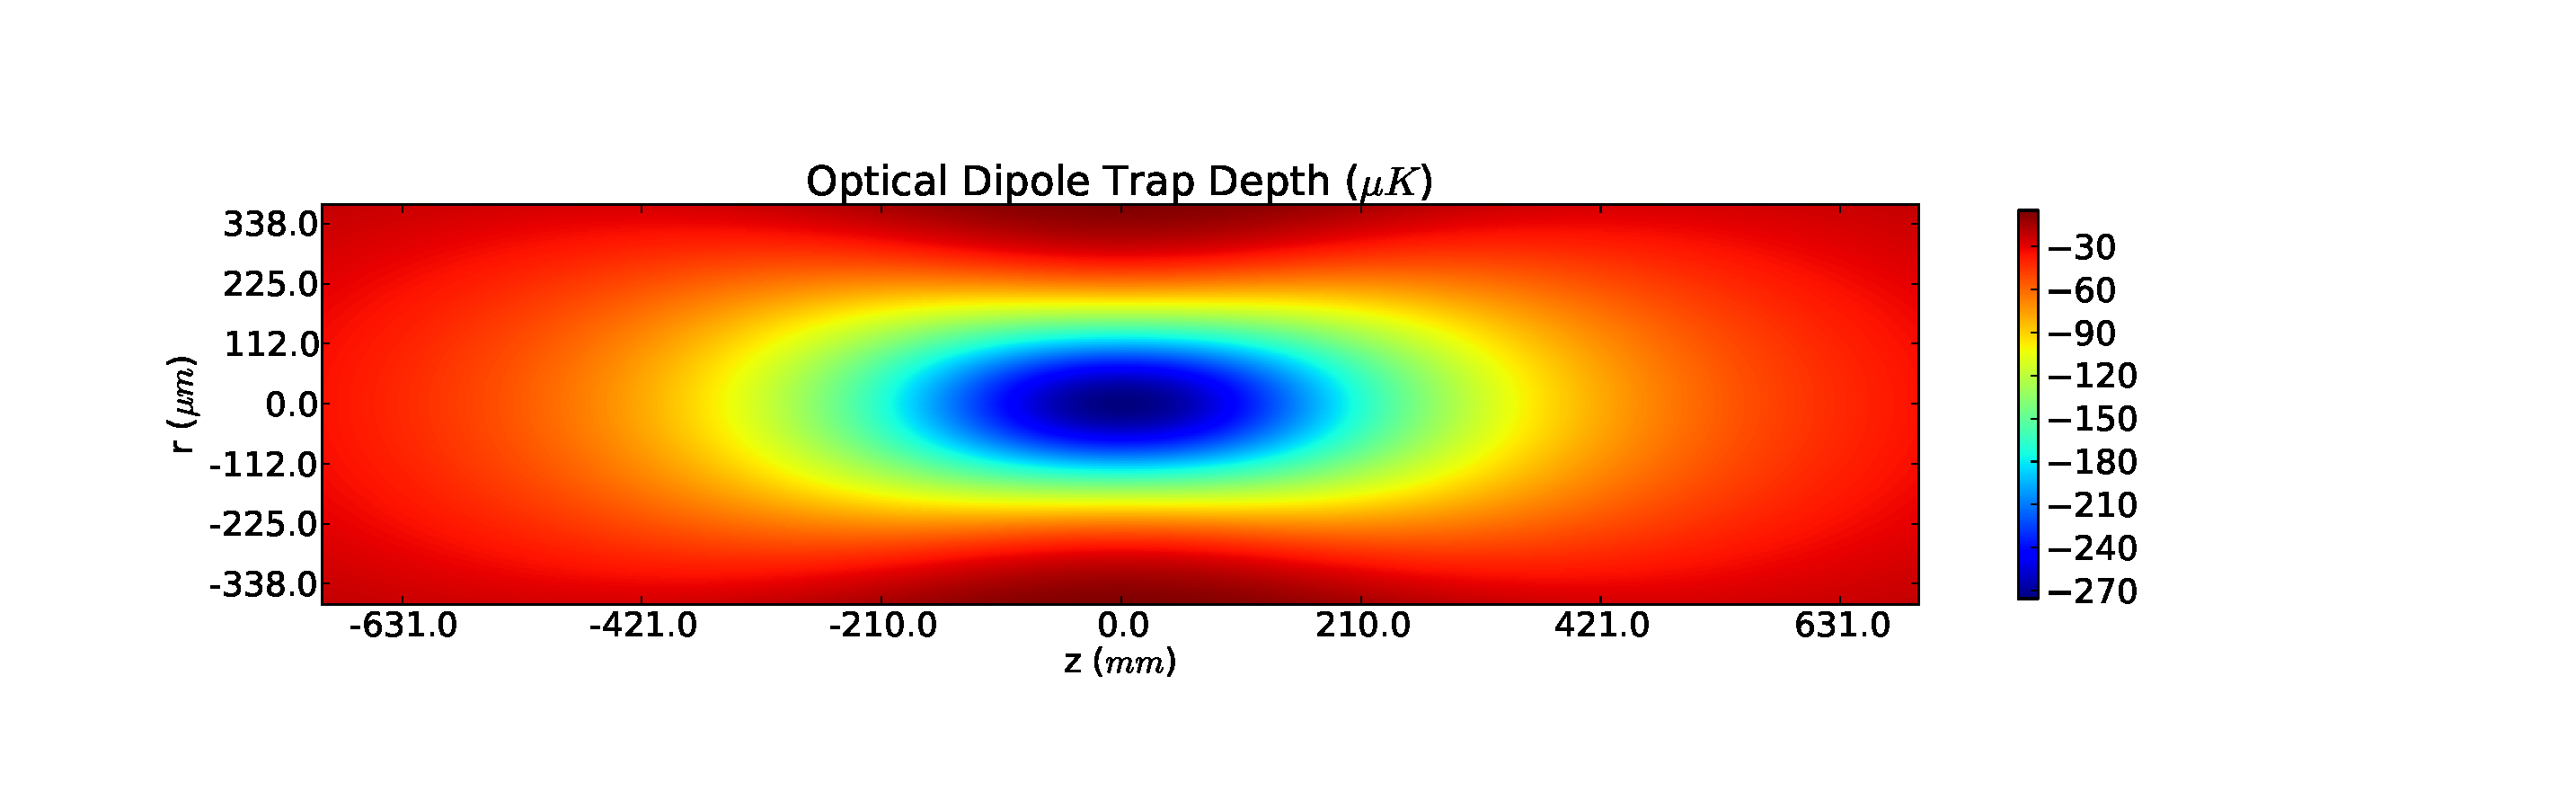
\includegraphics[width=\textwidth]{figs/2dtrapdepth.pdf}

\begin{subfigure}[b]{0.5\textwidth}
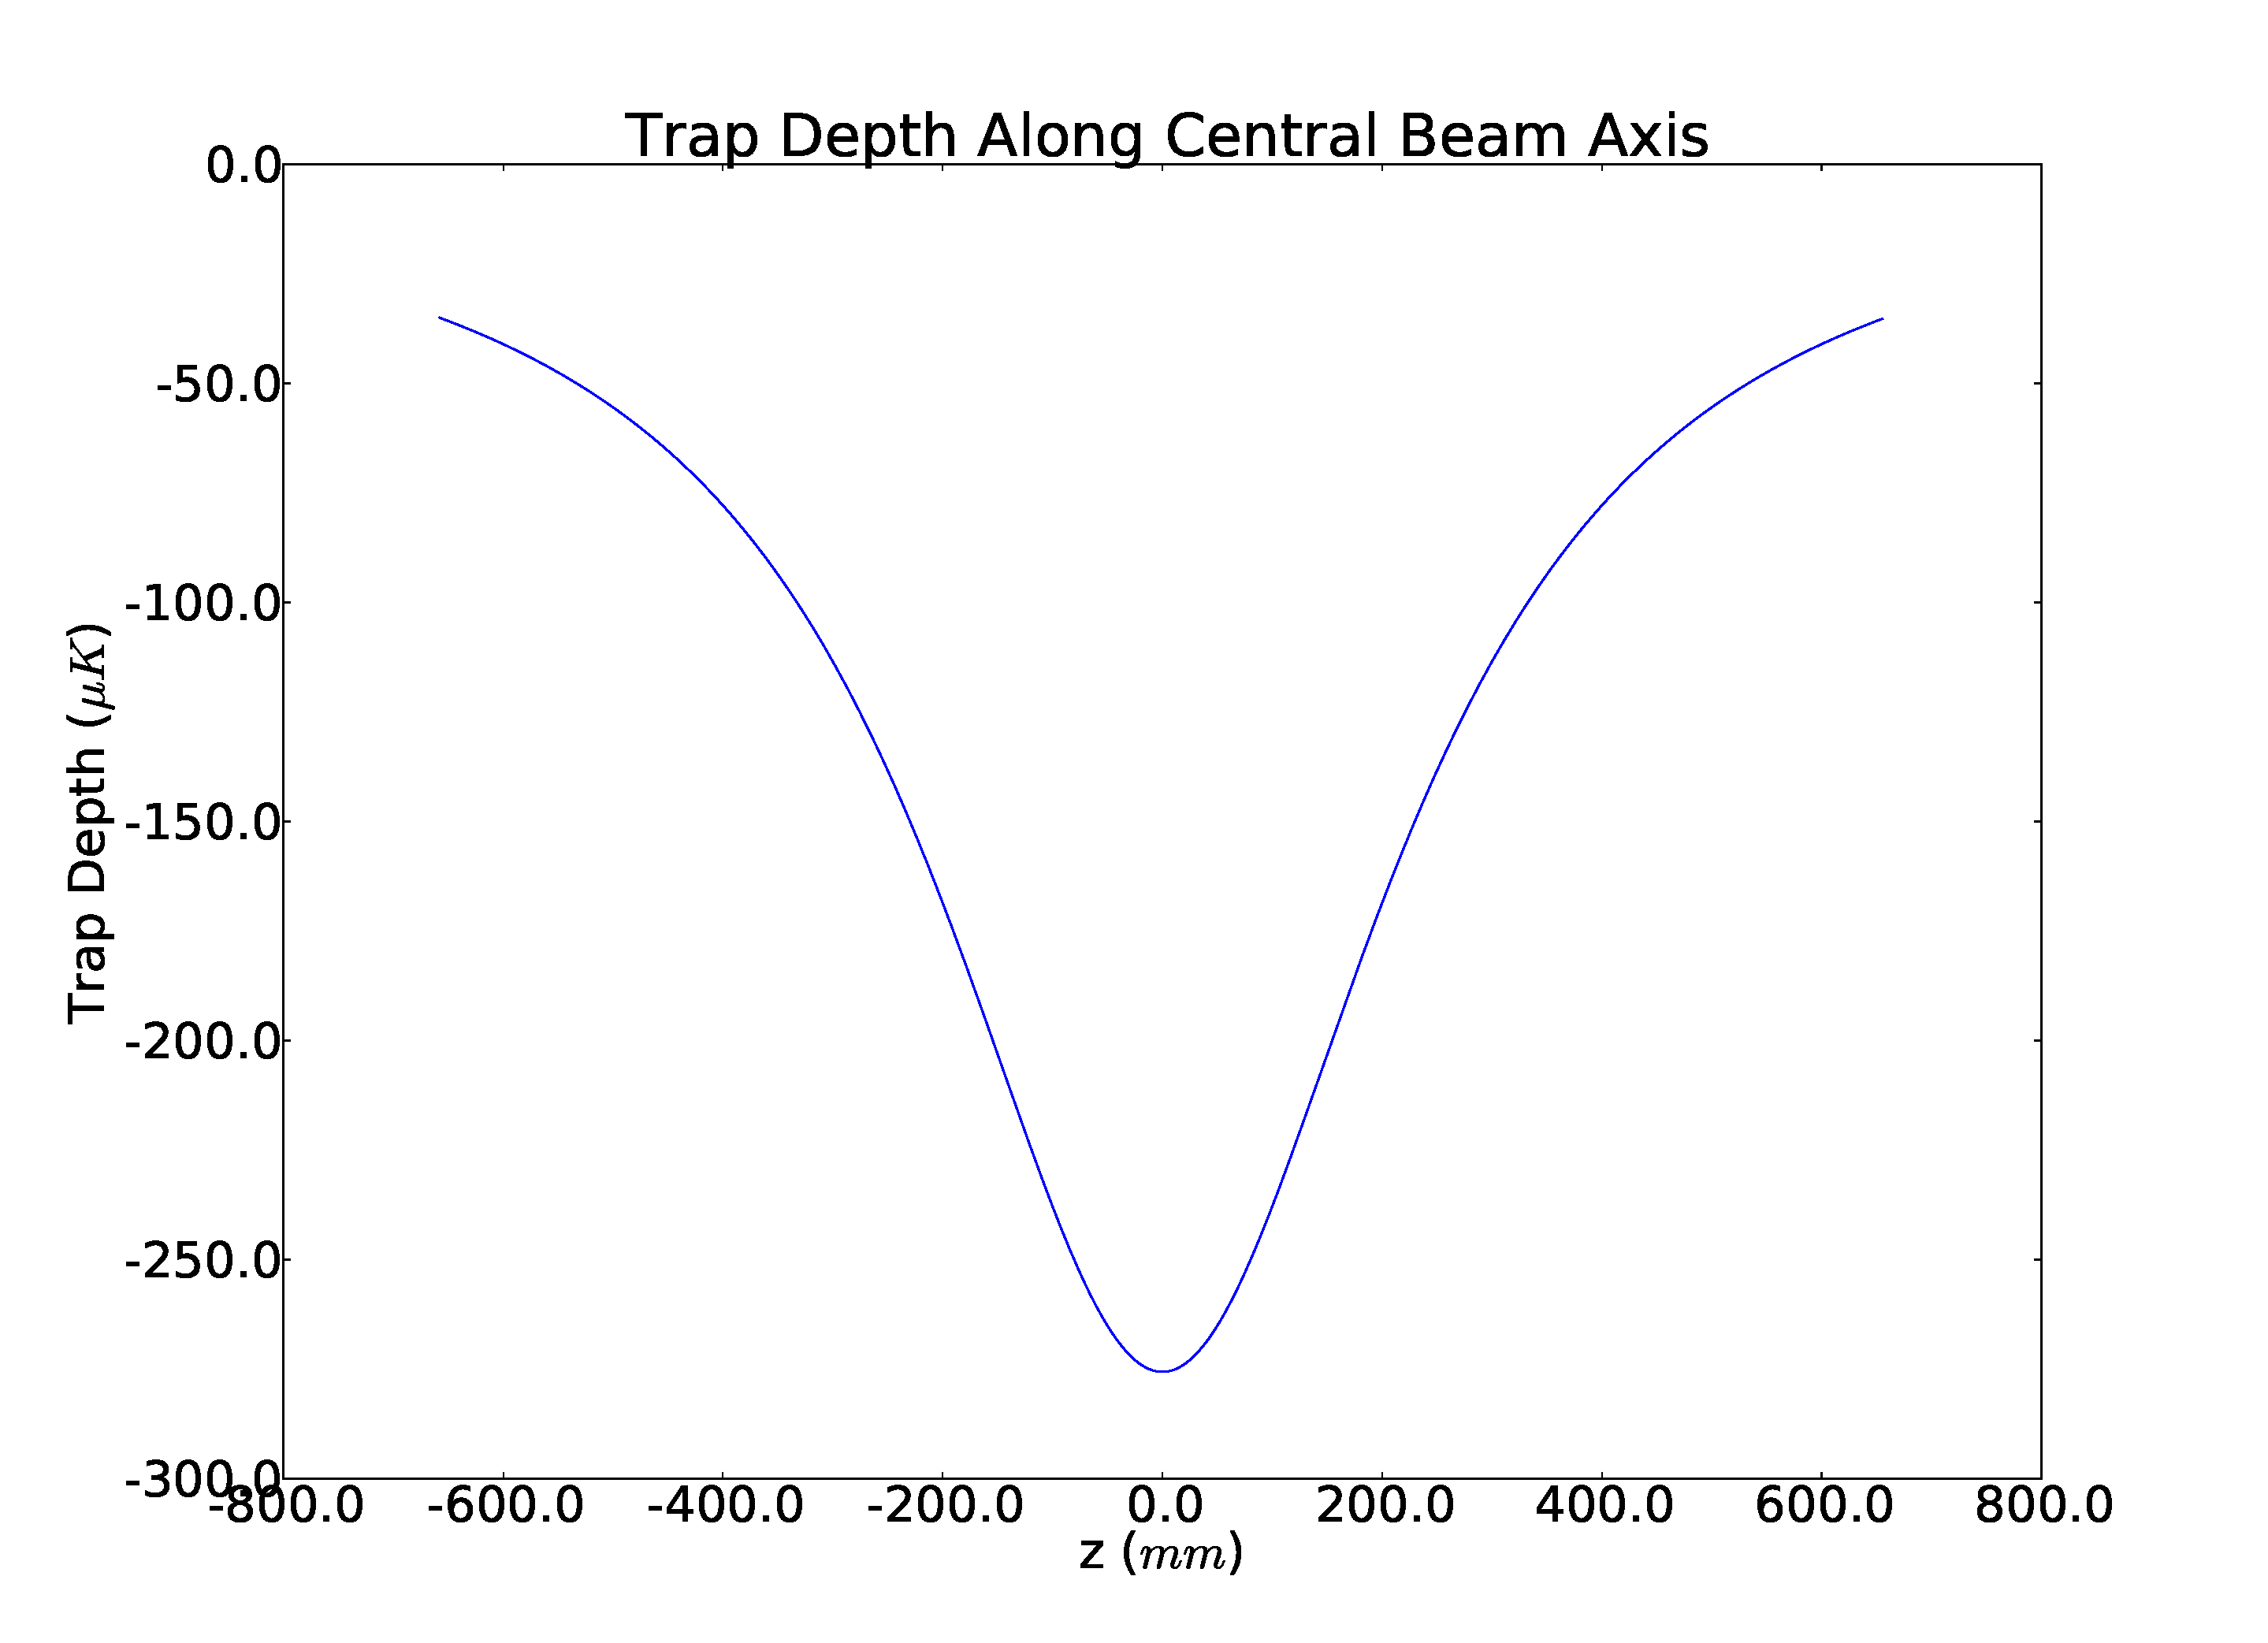
\includegraphics[width=\textwidth]{figs/longtrapdepth.pdf}
\end{subfigure}\begin{subfigure}[b]{0.5\textwidth}
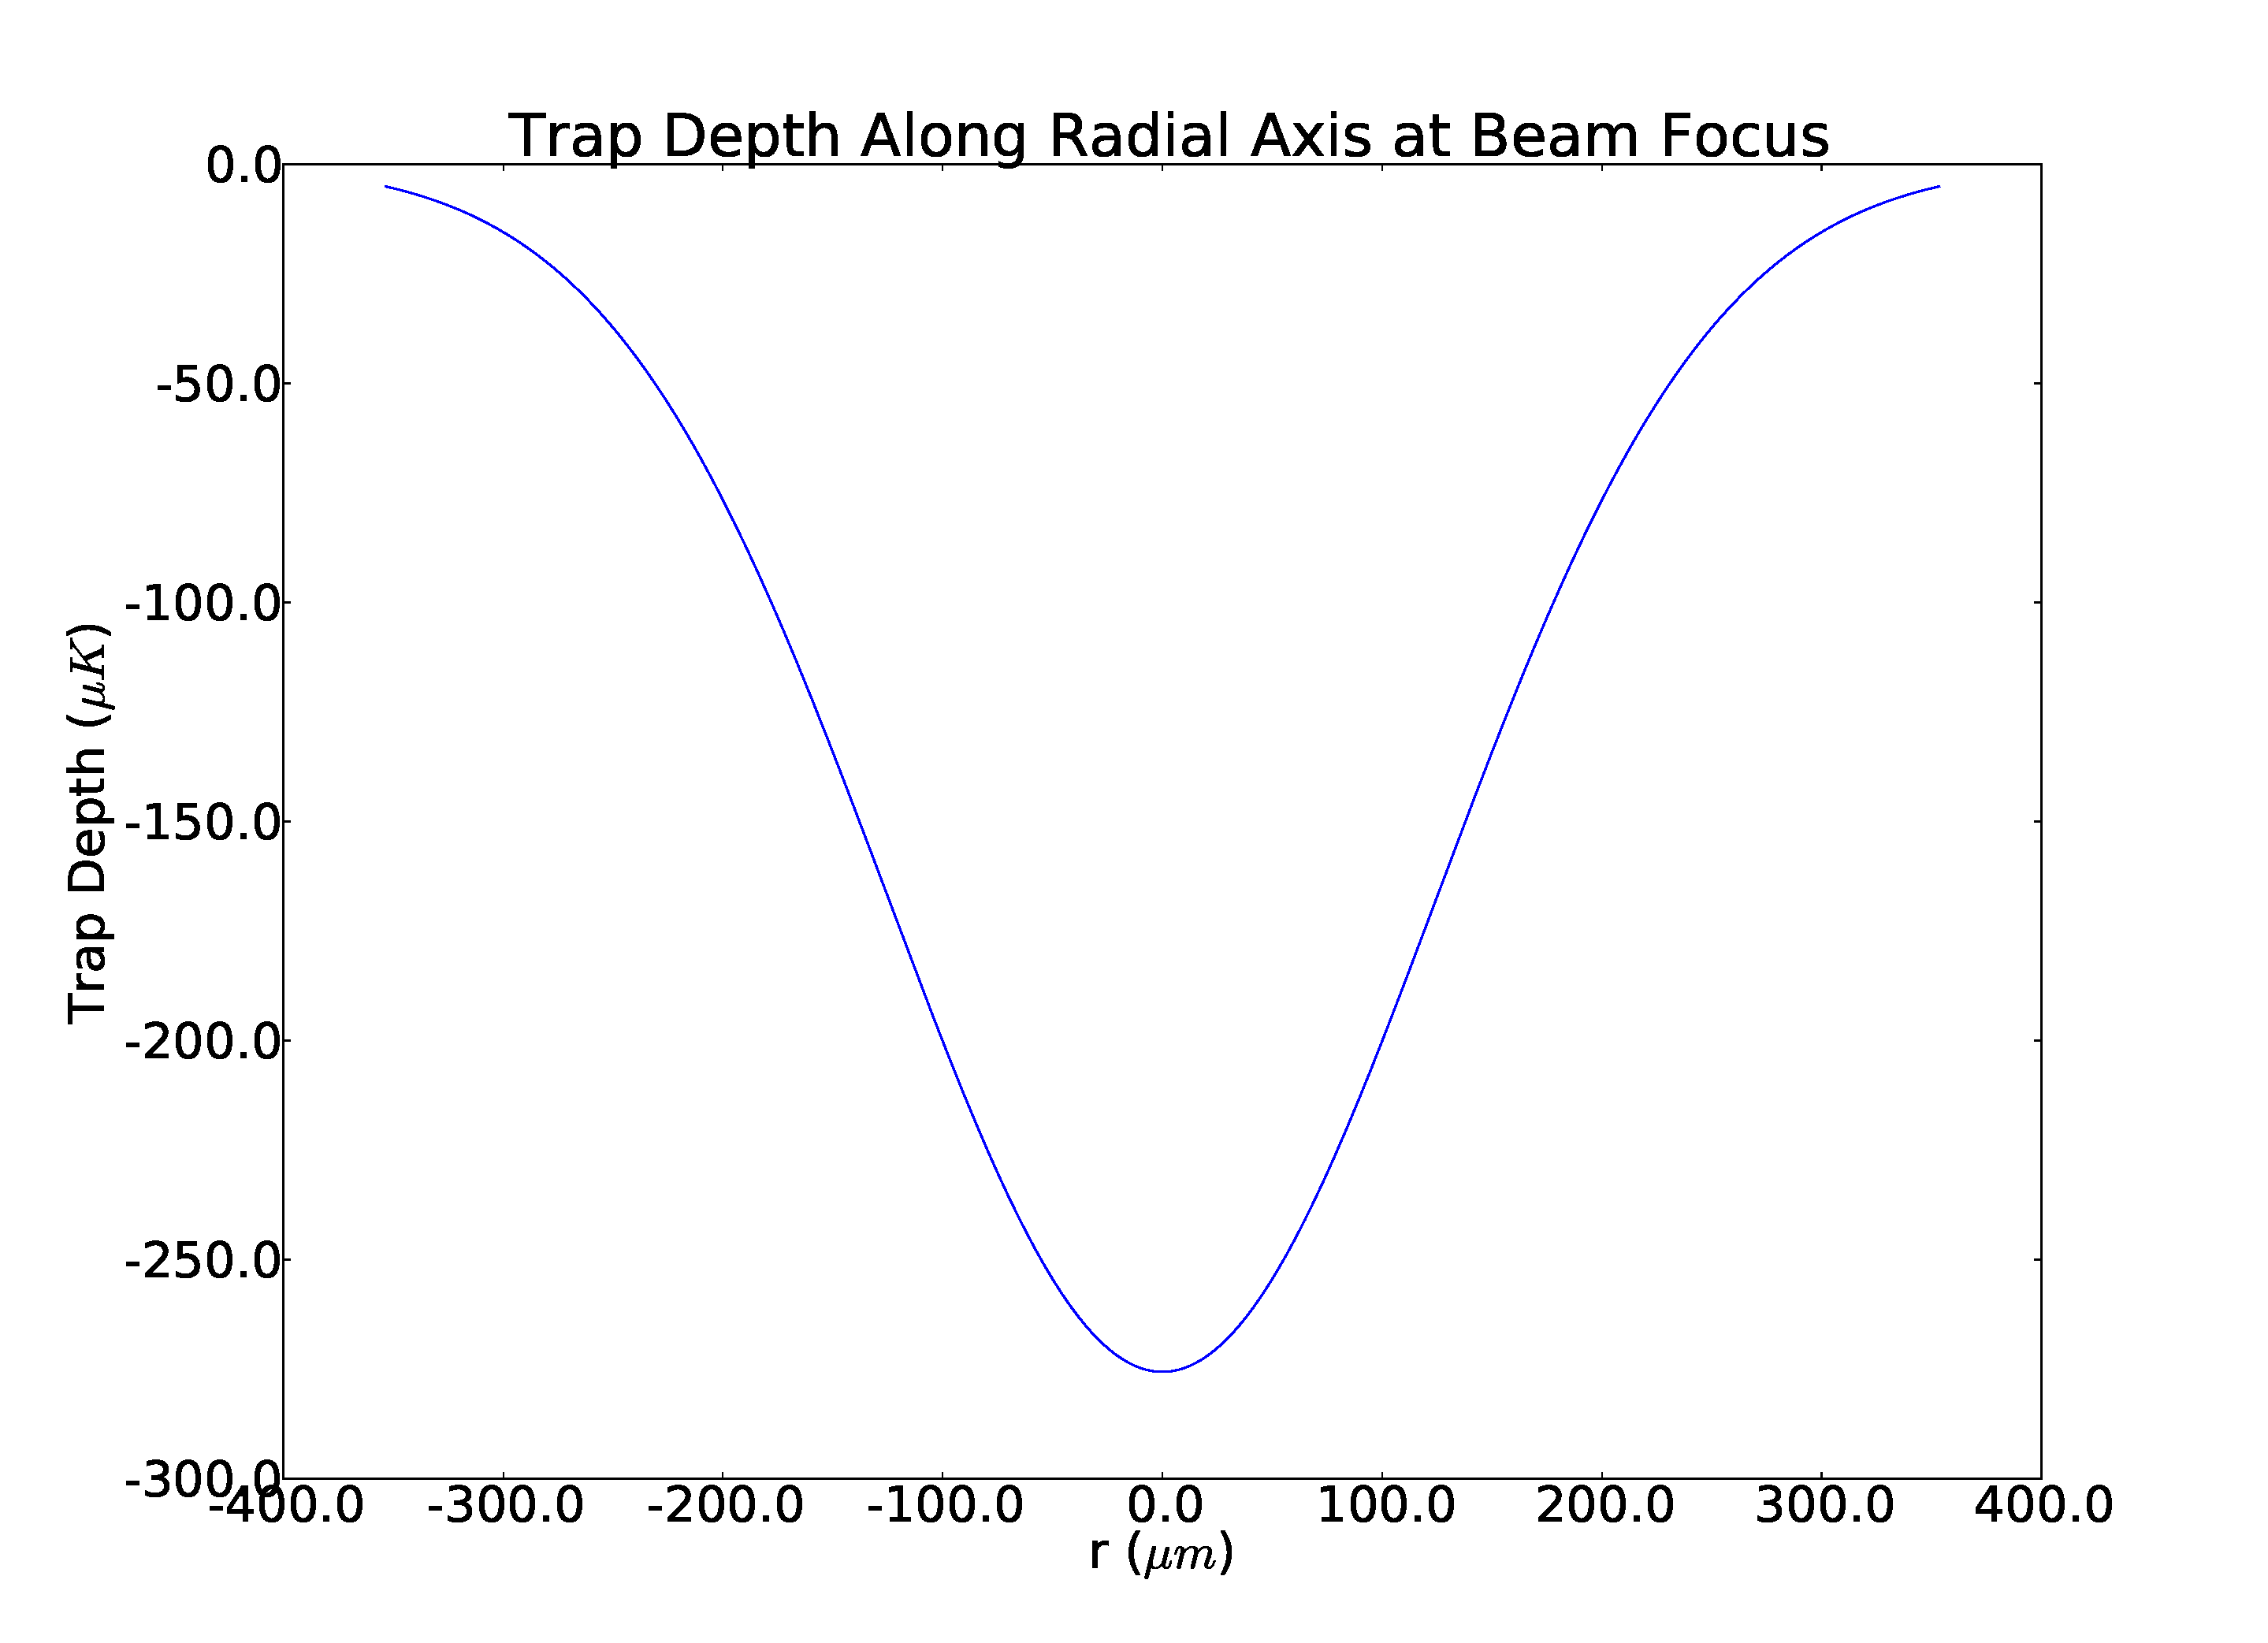
\includegraphics[width=\textwidth]{figs/radtrapdepth.pdf}
\end{subfigure}

\caption{The effective temperature of a single beam optical dipole trap is depicted here. The total power of the simulated beam is $500\,\unit{mW}$ with a detuning of $2\,\unit{nm}$ red of the $^{85}$Rb D2 resonance and a beam waist of $w_0=250\,\unit{\mu m}$. The top graph shows a cross section through the centre of the beam (note that the scale and units on each axis are different). The graph on the bottom left shows the axial trap depth in $\mu K$ at $r=0$ and the graph on the right shows the radial trap depth at $z=0$. The beam propagates in the $z$ direction.}
\label{fig:dipolepotential}
\end{figure}

\subsection{Trap Lifetime}
\label{lifetime_section}
The lifetime of an \gls{odt} is an important measure especially for \gls{bec} experiments, where lifetimes of seconds are routinely required\cite{cennini_bose-einstein_2003, kuppens_loading_2000, barrett_all-optical_2001}.

A simple model of the number of atoms in a trap over time, $N(t)$, can be expressed as
\begin{equation}
N(t) = N_0 e^{-\lambda t}
\end{equation}
where $N_0$ is the number of atoms at time $t=0$ and $\lambda$ is the decay rate.

\subsection{Configuration}

The simplest form of optical dipole trap consists of a single focussed Gaussian beam that traps atoms at the focus. These simple traps have been used since the 1980s\cite{chu_experimental_1986} and are frequently used to form \glspl{bec} and atom lasers\cite{chikkatur_continuous_2002, kleine_buning_slow_2010, lin_rapid_2009}.

Single beam traps have strong confinement in the direction perpendicular to beam propagation and relatively weak confinement along the beam. A trap with strong confinement in all directions can be created by crossing two beams. Crossed beam traps are also used frequently to produce \glspl{bec} \cite{couvert_quasi-monomode_2008, arnold_all-optical_2011, fu_bose-einstein_2011, barrett_all-optical_2001, xiong_evaporative_2010}. The polarisation of the two beam must be orthogonal in order to avoid the creation of standing waves.\label{odt_polarisation}

\begin{figure}[h]
\centering
\begin{subfigure}[b]{0.5\textwidth}
\centering
\begin{tikzpicture}
    \begin{scope}[scale=0.5]
        \shade[shading=radial, inner color=red, outer color=white] (-3,-1.581) -- (-3,1.581) -- plot[domain=-3:3] (\x, {0.3*sqrt(1+\x*\x)}) -- (3,1.581) -- (3,-1.581) -- plot[domain=3:-3] (\x, {-0.3*sqrt(1+\x*\x)}) -- cycle;
        \shade[ball color=brown] (0.0, 0.0) circle (0.05);
        \shade[ball color=brown] (0.025, 0.05) circle (0.05);
        \shade[ball color=brown] (-0.04, 0.1) circle (0.05);
        \shade[ball color=brown] (0.05, -0.025) circle (0.05);
        \shade[ball color=brown] (-0.05, -0.025) circle (0.05);
        \shade[ball color=brown] (-0.1, 0.05) circle (0.05);
        \shade[ball color=brown] (0.075, 0.115) circle (0.05);
        \shade[ball color=brown] (0.025, -0.1) circle (0.05);
        \shade[ball color=brown] (-0.085, -0.09) circle (0.05);
        \shade[ball color=brown] (0.11, 0.065) circle (0.05);
        \shade[ball color=brown] (0.10, 0.02) circle (0.05);
        \shade[ball color=brown] (0.00, 0.125) circle (0.05);

        \draw[-triangle 60] (-4,0) node[left] {Laser} -- (-3,0);

        \fill[gray, thick] (-2.4, 0) arc (0:15:5);
        \fill[gray, thick] (-2.4, 0) arc (0:-15:5) arc (195:165:5);
    \end{scope}
\end{tikzpicture}
\vspace{60pt}
\caption{A single beam optical dipole trap. A Gaussian laser propagates through a len and atoms are trapped axially at the focus.}
\end{subfigure}~~~\begin{subfigure}[b]{0.5\textwidth}
\centering
\begin{tikzpicture}
    \begin{scope}[scale=0.5]
        \shade[shading=radial, inner color=red, outer color=white] (-3,-1.581) -- (-3,1.581) -- plot[domain=-3:3] (\x, {0.15*sqrt(1+\x*\x)}) -- (3,1.581) -- (3,-1.581) -- plot[domain=3:-3] (\x, {-0.15*sqrt(1+\x*\x)}) -- cycle;
       \shade[shading=radial, inner color=red, outer color=white] (-1.581,-3) -- (1.581,-3) -- plot[domain=-3:3] ({0.15*sqrt(1+\x*\x)}, \x) -- (1.581,3) -- (-1.581,3) -- plot[domain=3:-3] ({-0.15*sqrt(1+\x*\x)}, \x) -- cycle;
        \shade[ball color=brown] (0.0, 0.0) circle (0.05);
        \shade[ball color=brown] (0.025, 0.05) circle (0.05);
        \shade[ball color=brown] (-0.04, 0.1) circle (0.05);
        \shade[ball color=brown] (0.05, -0.025) circle (0.05);
        \shade[ball color=brown] (-0.05, -0.025) circle (0.05);
        \shade[ball color=brown] (-0.1, 0.05) circle (0.05);
        \shade[ball color=brown] (0.075, 0.115) circle (0.05);
        \shade[ball color=brown] (0.025, -0.1) circle (0.05);
        \shade[ball color=brown] (-0.085, -0.09) circle (0.05);
        \shade[ball color=brown] (0.11, 0.065) circle (0.05);
        \shade[ball color=brown] (0.10, 0.02) circle (0.05);
        \shade[ball color=brown] (0.00, 0.125) circle (0.05);

        \draw[-triangle 60] (-4,0) node[left] {Laser} -- (-3,0);

        \fill[gray, thick] (-2.4, 0) arc (0:15:5);
        \fill[gray, thick] (-2.4, 0) arc (0:-15:5) arc (195:165:5);

        \draw[-triangle 60] (0,-4) node[below] {Laser} -- (0,-3);

        \fill[gray, thick] (0, -2.4) arc (90:105:5);
        \fill[gray, thick] (0, -2.4) arc (90:75:5) arc (-75:-105:5);
    \end{scope}
\end{tikzpicture}
\caption{A crossed beam optical dipole trap. Two Gaussian lasers propagate through lens and cross at the focal points. Atoms are trapped in all directions at the foci.}
\end{subfigure}
\end{figure}

Good trapping in all directions is required for the \gls{caes} so a crossed beam setup has been used.

\section{Imaging}

Two types of imaging were used to observethe oepration of the \gls{odt} and to optimise its performance.

\subsection{Fluorescence Imaging}

Resonant or near-resonant photons passing through atom clouds (such as the optical molasses lasers in a \gls{mot} or a specific probe beam) will be absorbed and re-emitted in a random direction. These scattered photons can be easily detected to form images. This method allows imaging along any axis. The signal is rather weak however since the scattered photons are equally distributed in all directions so only a small portion will reach the detector which can make precise imaging more difficult. Due to the strong interaction of the laser light with the atoms this is a destructive imaging method.

\begin{figure}[h]
\centering
\begin{tikzpicture}
    \begin{scope}[decoration={snake,amplitude=.4mm,segment length=2mm,post length=1mm}]
        \draw (-3.2, 0) node[rotate=90] {Probe Laser};
        \shade[bottom color=red, top color=white] (-3,0.35) rectangle (3, 0.75);
        \shade[top color=red] (-3,-0.34) rectangle (3, -0.75);
        \fill[color=red] (-3, 0.36) rectangle (3, -0.35);

        \draw[thick, -triangle 60] (-2.5, 0) -- (-1.5, 0);

        \shade[top color=red] (-0.01,-0.01) rectangle (3, 0.35);
        \shade[bottom color=red, top color=white] (-0.01,0.01) rectangle (3, -0.35);

        \fill[gray, thick] (0, -0.8) arc (90:105:5);
        \fill[gray, thick] (0, -0.8) arc (90:75:5) arc (-75:-105:5);

        \draw[thick, decorate,blue,->] (0,0) -- ++(0:1.25);
        \draw[thick, decorate,blue,->] (0,0) -- ++(30:1.25);
        \draw[thick, decorate,blue,->] (0,0) -- ++(60:0.866);
        \draw[thick, decorate,blue,->] (0,0) -- ++(90:0.75);
        \draw[thick, decorate,blue,->] (0,0) -- ++(120:0.866);
        \draw[thick, decorate,blue,->] (0,0) -- ++(150:1.25);
        \draw[thick, decorate,blue,->] (0,0) -- ++(180:1.25);
        \draw[thick, decorate,blue,->] (0,0) -- ++(210:1.25);
        \draw[thick, decorate,blue,->] (0,0) -- ++(240:1.25);
        \draw[thick, decorate,blue,->] (0,0) -- ++(270:1.2);
        \draw[thick, decorate,blue,->] (0,0) -- ++(300:1.25);
        \draw[thick, decorate,blue,->] (0,0) -- ++(330:1.25);

%        \draw[thick, decorate,blue,->] (-3,-1.7) --
%            node[above, black] {\small Fluorescence} ++(0:1.25);

        \filldraw[fill=gray, draw=black] (-1,-1.3) rectangle
            node[color=black] {Detector} (1,-1.8);
        \filldraw[fill=gray, draw=black] (-0.9,-1.2) rectangle (0.9, -1.3);

        \draw (0, 0.75) node[above] {Atom Cloud};
        \shade[ball color=brown] (0.0, 0.0) circle (0.1);
        \shade[ball color=brown] (0.05, 0.1) circle (0.1);
        \shade[ball color=brown] (-0.08, 0.2) circle (0.1);
        \shade[ball color=brown] (0.1, -0.05) circle (0.1);
        \shade[ball color=brown] (-0.1, -0.05) circle (0.1);
        \shade[ball color=brown] (-0.2, 0.1) circle (0.1);
        \shade[ball color=brown] (0.15, 0.23) circle (0.1);
        \shade[ball color=brown] (0.05, -0.2) circle (0.1);
        \shade[ball color=brown] (-0.17, -0.18) circle (0.1);
        \shade[ball color=brown] (0.22, 0.13) circle (0.1);
        \shade[ball color=brown] (0.20, 0.04) circle (0.1);
        \shade[ball color=brown] (0.00, 0.25) circle (0.1);
    \end{scope}
\end{tikzpicture}
\caption{In fluorescence imaging, light from the on-resonance probe beam is absorbed by the atoms and then reemitted in all directions as fluorescence. This light is captured by the detector.}
\end{figure}

\begin{figure}[h]
\centering

\begin{tikzpicture}
    \node[anchor=south west,inner sep=0] (image) at (0,0) {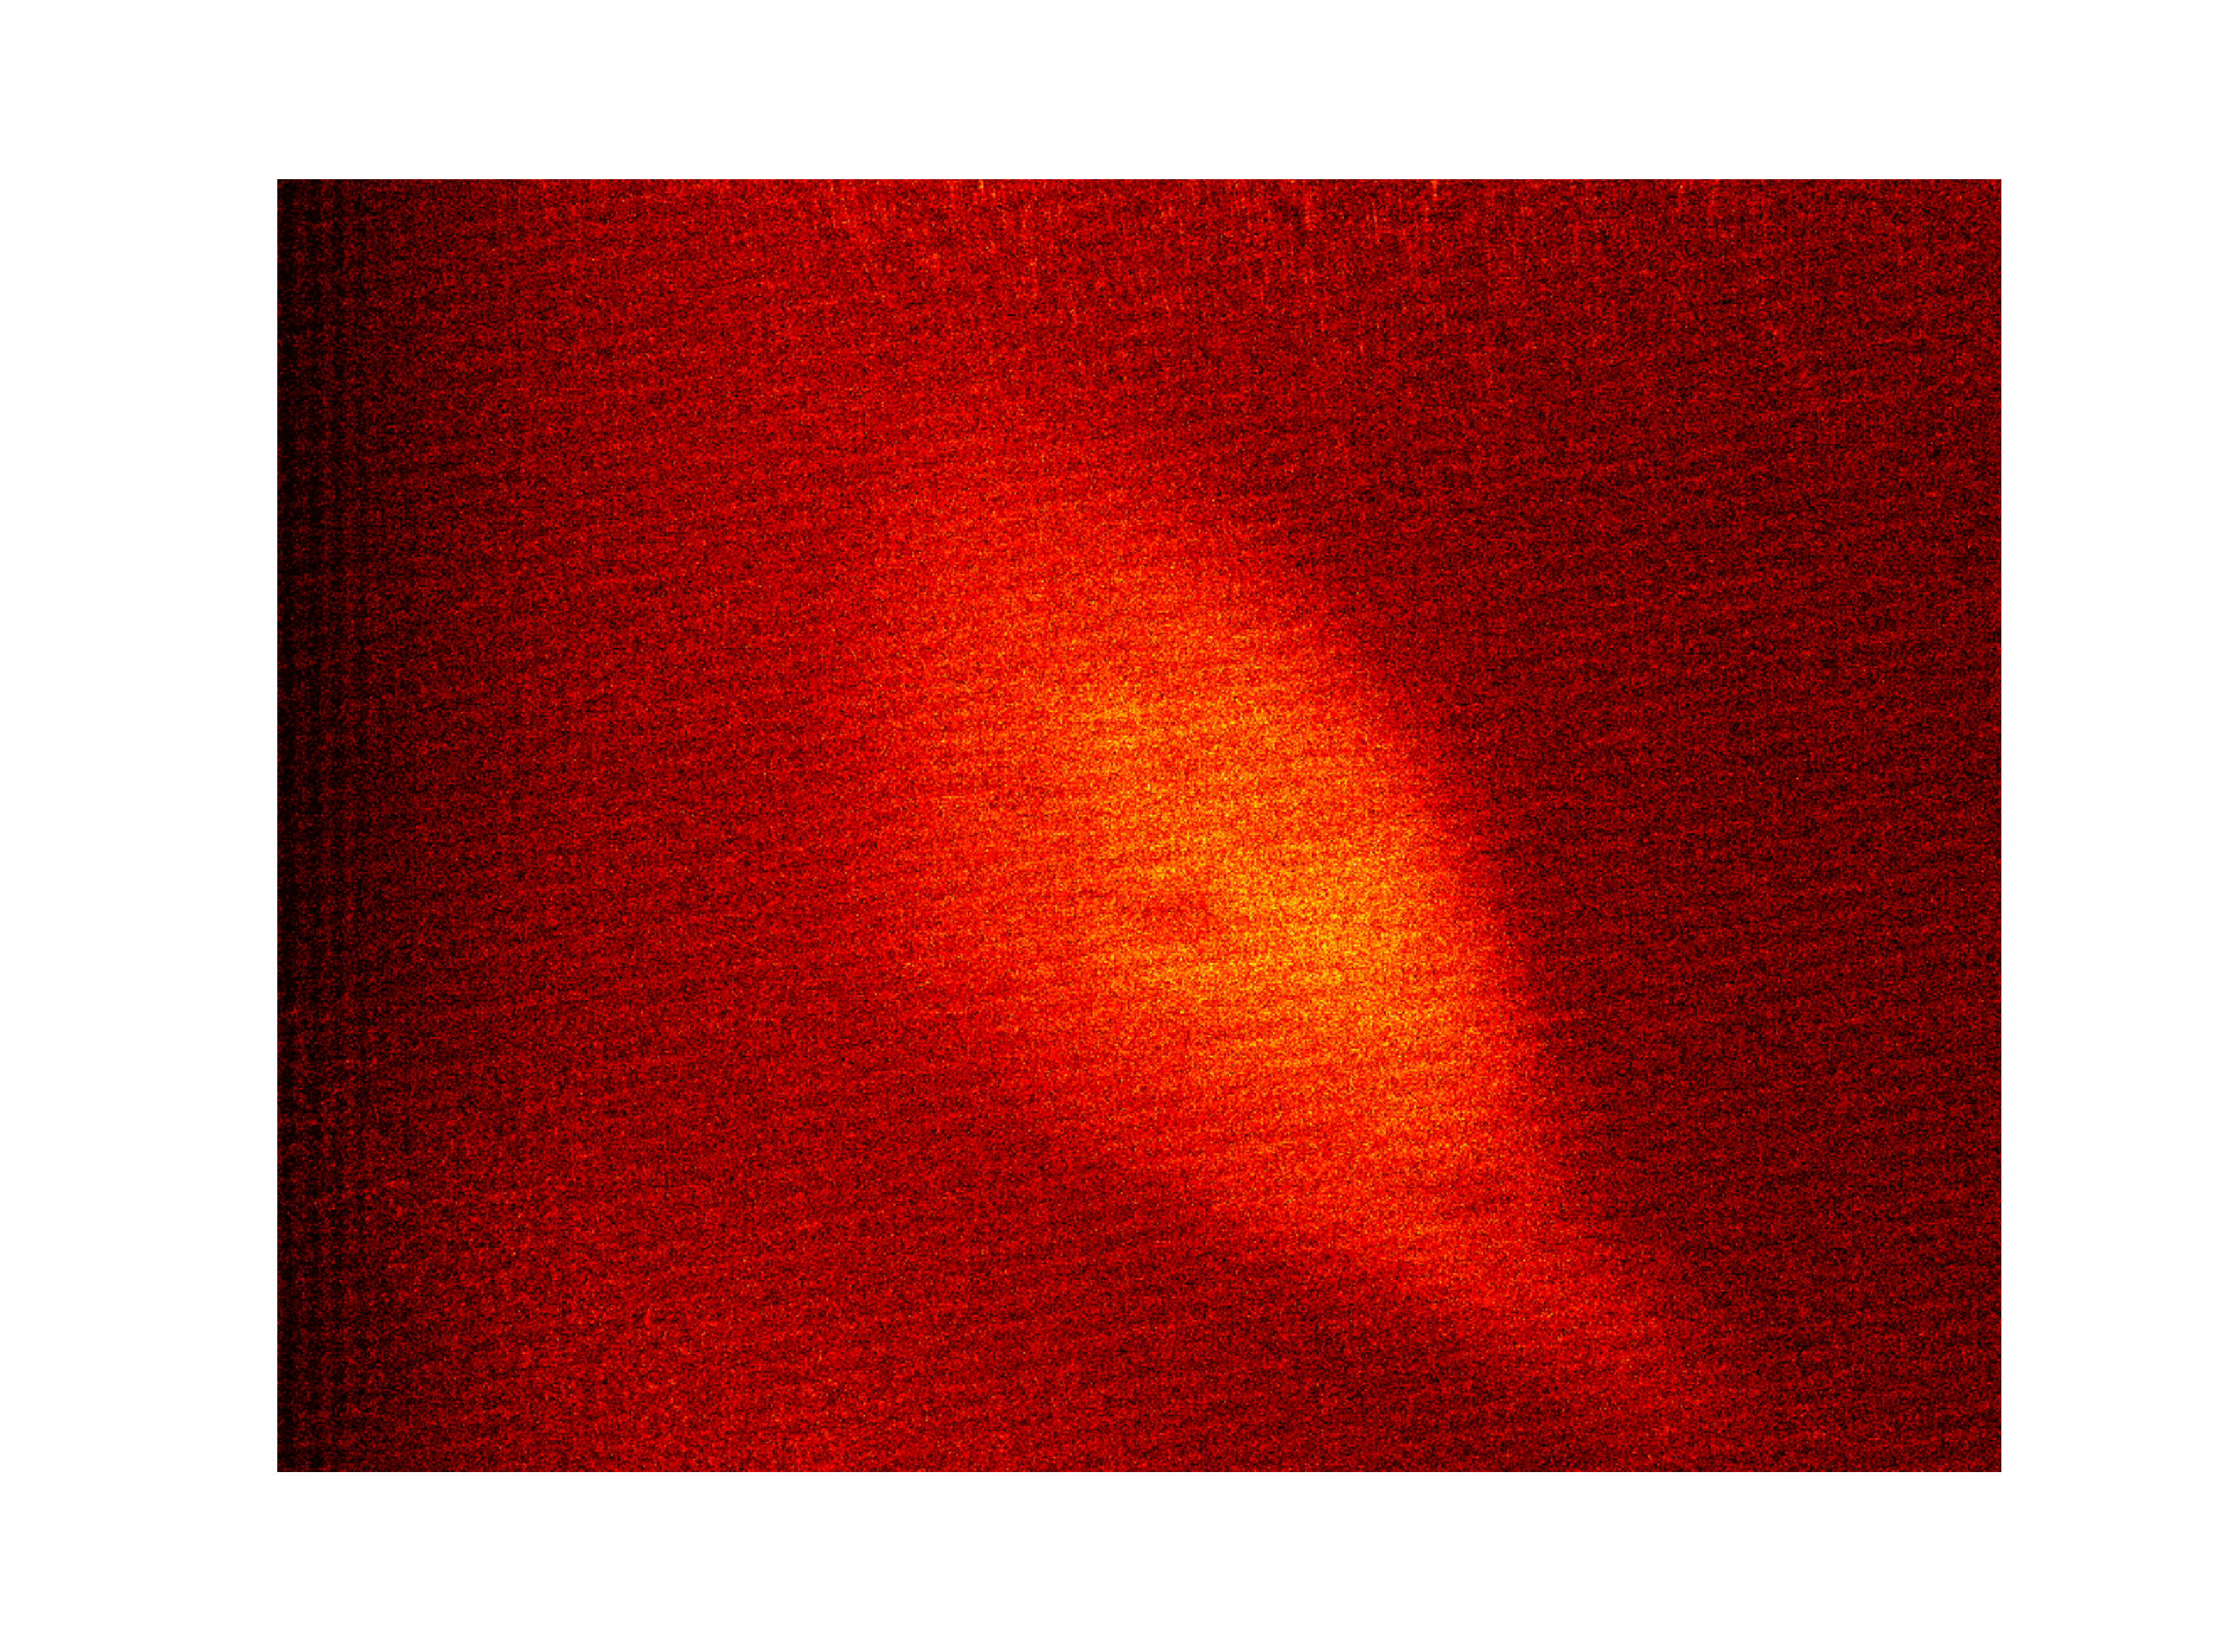
\includegraphics[width=0.3\textwidth]{figs/fluorescence.pdf}};
    \begin{scope}[x={(image.south east)},y={(image.north west)}]
        \draw[white,thick] (0.2,0.15) -- node[above]{\large $5\,\unit{mm}$} (0.49524,0.15);
    \end{scope}
\end{tikzpicture}

\caption{A short exposure, false colour fluorescence image of the MOT.}
\end{figure}

Fluorescence imaging is used in the Melbourne \gls{caes} to view the \gls{mot} but is not practical for use with atoms trapped in an \gls{odt} due to the very  small number of atoms in the \gls{odt}

\subsection{Absorption Imaging}

Absorption imaging is another destructive imaging method that makes use of an on-resonance probe laser. A collimated probe laser is directed through the atoms and onto the detector. The photons will be absorbed and reemitted in random directions. After the light has passed through the atoms a `shadow' due to the photon absorption by the atoms will be left in the probe beam. The `shadow' is used to create an absorption image. The signal from absorption imaging is much stronger than that for fluorescence.

\begin{figure}[h]
\centering
\begin{tikzpicture}
    \begin{scope}
        \draw (-3.2, 0) node[rotate=90] {Probe Beam};
        \shade[bottom color=red, top color=white] (-3,0.35) rectangle (3, 0.75);
        \shade[top color=red] (-3,-0.34) rectangle (3, -0.75);
        \fill[color=red] (-3, 0.36) rectangle (3, -0.35);

        \draw[thick, -triangle 60] (-2.5, 0) -- (-1.5, 0);

        \shade[top color=red] (-0.01,-0.01) rectangle (3, 0.35);
        \shade[bottom color=red, top color=white] (-0.01,0.01) rectangle (3, -0.35);

        \fill[gray, thick] (2.7, 0) arc (0:15:5);
        \fill[gray, thick] (2.7, 0) arc (0:-15:5) arc (195:165:5);

        \filldraw[fill=gray, draw=black] (3,1) rectangle
            node[color=black, rotate=90] {Detector} (3.5, -1);
        \filldraw[fill=gray, draw=black] (2.9,0.8) rectangle (3, -0.8);

        \draw (0, 0.75) node[above] {Atom Cloud};
        \shade[ball color=brown] (0.0, 0.0) circle (0.1);
        \shade[ball color=brown] (0.05, 0.1) circle (0.1);
        \shade[ball color=brown] (-0.08, 0.2) circle (0.1);
        \shade[ball color=brown] (0.1, -0.05) circle (0.1);
        \shade[ball color=brown] (-0.1, -0.05) circle (0.1);
        \shade[ball color=brown] (-0.2, 0.1) circle (0.1);
        \shade[ball color=brown] (0.15, 0.23) circle (0.1);
        \shade[ball color=brown] (0.05, -0.2) circle (0.1);
        \shade[ball color=brown] (-0.17, -0.18) circle (0.1);
        \shade[ball color=brown] (0.22, 0.13) circle (0.1);
        \shade[ball color=brown] (0.20, 0.04) circle (0.1);
        \shade[ball color=brown] (0.00, 0.25) circle (0.1);

    \end{scope}
\end{tikzpicture}
\caption{The on-resonance probe beam propagating from left to right passes through the atom cloud. The atoms absorb some of the light and the shadow is visible on the detector.}
\end{figure}

\begin{figure}[h]
\centering
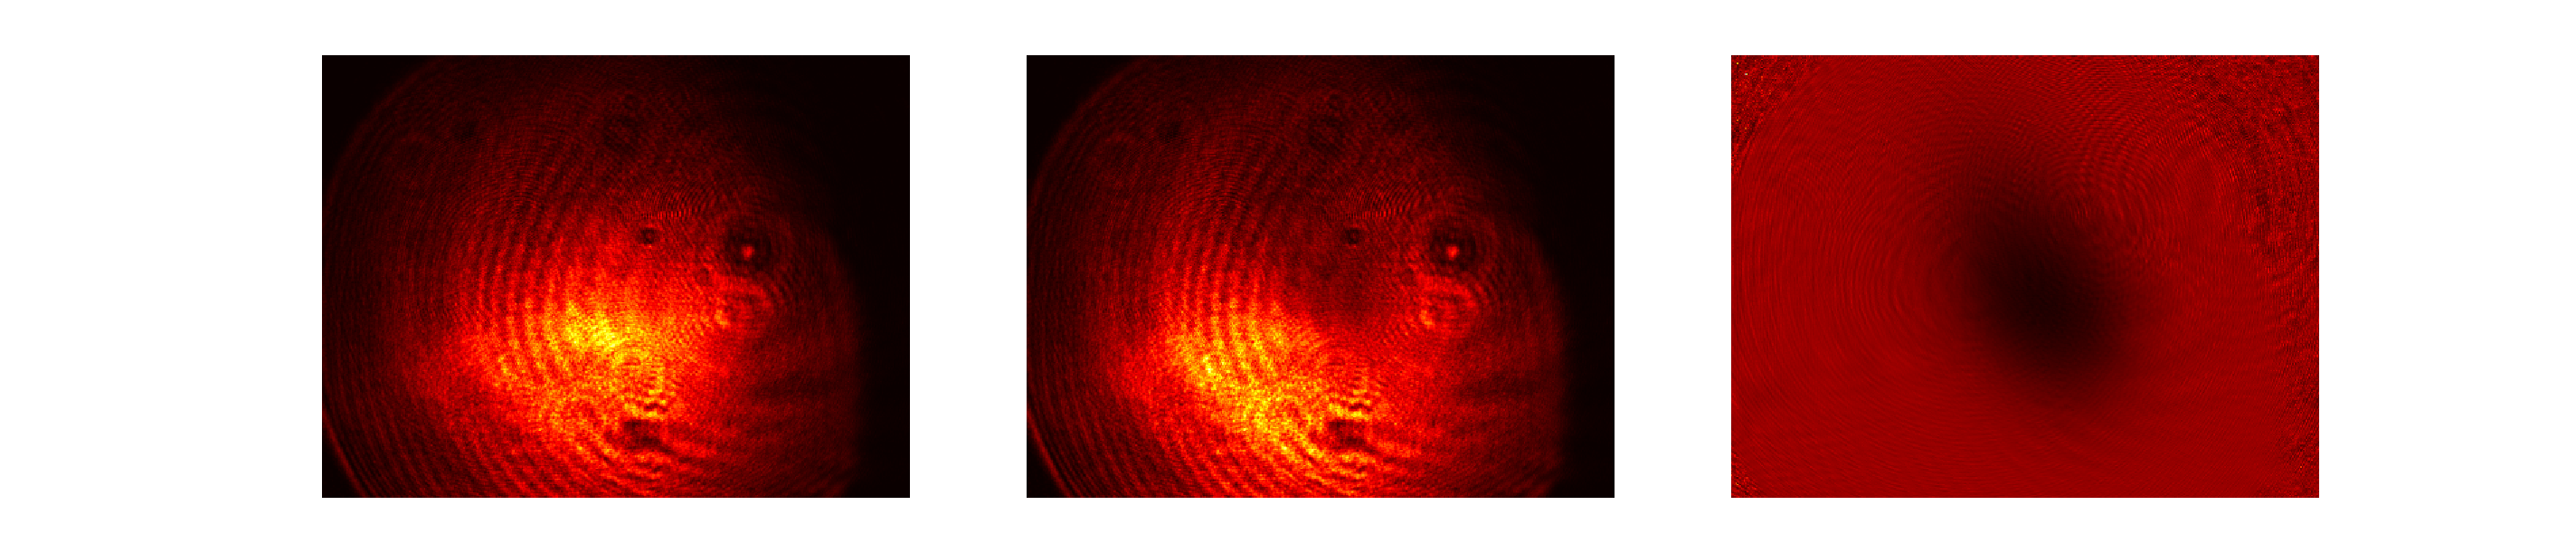
\includegraphics[width=18cm]{figs/absorptionexample.pdf}
\caption{The above images are an example of absorption imaging.  The image on the left is that of the on-resonance probe beam taken while the magnetic trapping of the magneto-optic trap was turned off and no atoms were trapped. The centre image shows the probe beam after it had passed through the atom-cloud of the normal magneto-optic trap and the corresponding shadow is clearly visible. The transmission function of the atoms (see equation \ref{eq:transmission_function_1}) is shown in the right image.}
\label{fig:absorption_example}
\end{figure}

\subsection{Absorption Imaging Analysis}
\label{sec:absorption_imaging}
If $I_0$ and $I$ are images taken with and without atoms present then then the transmission function for the atoms, $G$, can be calculated with

\begin{equation}
I = G I_0.
\end{equation}
\begin{equation}\label{eq:transmission_function_1}
G = \frac{I}{I_0}.
\end{equation}
Each point in $G$ corresponds to the integrated column density of the atoms in the cloud at that radial location and this information can be used to determine a number of different metrics such as the temperature of the atoms and the total number of atoms.

\subsection{MOT Temperature}
\label{temp_measurement}
An atomic spatial density distribution in an ideal \gls{mot} atom cloud should be Gaussian. The two-dimensional density can be described by
\begin{equation}\label{eq:gaussian_density}
\rho (x, y) = \rho_0\exp\left(\frac{x^2}{\sigma_x^2} + \frac{y^2}{\sigma_y^2}\right)
\end{equation}
where $\rho_0$ is the central density and $\sigma_x$ and $\sigma_y$ are the 1/e radii of the distribution. This assumes that any ellipticity is aligned with the $x$ and $y$ axes.

If the trapping lasers and magnetic fields are turned off the atom-cloud begins to expand thermally. The r.m.s. thermal velocity, $v_0$, is related to the temperature of the cloud, $T$, via \cite{sheludko_shaped_2010}
\begin{equation}\label{eq:temp_velocity}
v_0 = \sqrt{\frac{2k_BT}{m_{Rb}}}
\end{equation}
where $k_B$ is Boltzmann's constant and $m_{Rb}$ is the mass of rubidium. The 1/e radius of the atom cloud, $r$, at time $t$ after release is given by
\begin{equation}\label{eq:cloud_radius}
r(t) = \sqrt{r_0^2 + (v_0t)^2}.
\end{equation}
Here $r_0$ is the initial 1/e radius of the cloud.

The temperature can be calculated by taking a number of absorption images for various values of $t$ and then fitting each of the atomic distributions to equation \ref{eq:gaussian_density}. The various cloud radii can be fitted to equation \ref{eq:cloud_radius} and a temperature can be calculated with equation \ref{eq:temp_velocity}.

\subsection{Atom Count}
\label{atom_count}
%http://qwiki.stanford.edu/index.php/BEC_How_To

It is useful to know the number of atoms in a given absorption image. To do this we need to know the magnification of the optical system in front of the detector as well as the power of the probe laser.

As the probe laser traverses through the atoms cloud its intensity obeys Beer's law\cite{foot_atomic_2005}
\begin{equation}\label{eq:beers_law}
I(x, y) = I_0(x, y)e^{-D(x, y)}
\end{equation}
where $I_0(x, y)$ is the intensity of the beam before the cloud, $I(x, y)$ is the intensity after the cloud and $D(x, y)$ is the optical depth along the probe beam's axis. The coordinates $(x, y)$ denote a given position in the plane perpendicular to the probe beam. The optical density is given by
\begin{equation}\label{eq:optical_density}
D(x, y) = \sigma \int_{-\infty}^{\infty}n(x, y, z)dz.
\end{equation}
Here $\sigma$ is the absorption cross-section and $n(x, y, z)$ is the atomic density distribution.

Using equations \ref{eq:beers_law} and \ref{eq:optical_density} we find
\begin{equation}
D(x, y) = -\ln(\frac{I}{I_0}) = \sigma \int_{-\infty}^{\infty} n(x, y, z) dz.
\end{equation}

Integrating across the image we obtain
\begin{equation}
\int_{-\infty}^{\infty} \int_{-\infty}^{\infty} \frac{1}{\sigma}D(x, y) dx dy = N.
\end{equation}
Practically $I$, $I_0$ and $D(x, y)$ will be two dimensional arrays of pixels, so the integrals can be rewritten as sums over the pixels giving
\begin{equation}\label{eq:atom_sum}
N = \sum_{(x, y)} \frac{1}{\sigma}D(x, y)A_{pixel}
\end{equation}
where $A_{pixel}$ is the scaled area of the a pixel. Here `scaled' implies that the magnification of the optical system has been taken into account.

The absorption cross-section is given by \cite{steck_rubidium_2001}
\begin{equation}\label{eq:cross_section}
\sigma = \frac{\sigma_0}{1+4(\Delta/\Gamma)^2 + (I/I_s)}
\end{equation}
where $\Delta$ is the frequency detuning of the pump light ($\Delta=0$ for on-resonant light) and $\sigma_0$ is the on-resonance, low-intensity  cross-section
\begin{equation}
\sigma_0 = \frac{\hbar\omega\Gamma}{2I_s}.
\end{equation}

Combining equations \ref{eq:atom_sum} and \ref{eq:cross_section} provides
\begin{equation}
\label{eq:atom_count}
N = -\frac{A_{pixel}}{\sigma_0} \sum_{(x, y)} (1+(I(x, y)/I_s)) \ln\left(\frac{I(x, y)}{I_0(x, y)}\right)
\end{equation}
for on-resonant light. If on-resonant light with an intensity much less than the saturation intensity is used then $\sigma \approx \sigma_0$ and
\begin{equation}
N = -\frac{A_{pixel}}{\sigma_0} \sum_{(x, y)} \ln\left(\frac{I(x, y)}{I_0(x, y)}\right).
\end{equation}

